\documentclass[twocolumn]{article}

\usepackage[backend=biber]{biblatex}
\usepackage[margin=0.7in]{geometry}
\usepackage[font={normalsize,it}]{caption}
\usepackage{titlesec}
\usepackage{graphicx}

\addbibresource{references.bib}

\renewcommand{\thesection}{\Roman{section}}
\renewcommand{\thesubsection}{\Alph{subsection}}

\titleformat{\subsection}{\small\it}{\thesubsection.}{0.9em}{}
\titleformat{\section}{\large\sc\filcenter}{\thesection.}{1em}{}

\begin{document}

\twocolumn[
  \begin{center}

\vspace{1.7cm}

\begin{Huge}
Slum Detection using Multiclass Land Cover in Bangalore
\end{Huge}


\vspace{1.5cm}

Derk Barten\\
11043075

\vspace{1.5cm}

Honors Bachelor thesis extention\\
Credits: 6 EC

\vspace{0.5cm}

Bachelor Opleiding Kunstmatige Intelligentie

\vspace{0.25cm}

University of Amsterdam\\
Faculty of Science\\
Science Park 904\\
1098 XH Amsterdam

\vspace{4cm}

\emph{Supervisor}\\
Dr. Debraj Roy

\vspace{0.25cm}

Department of Computational Science\\
Faculty of Science\\
University of Amsterdam\\
Science Park 904\\
1098 XH  Amsterdam

\vspace{1.5cm}

\today

\end{center}


]
\clearpage

\section{Introduction}

Informal housing is a common issue faced by cities in developing countries. Inhabitants of informal regions, commonly named as slums, have less social economic opportunities and a lower quality of life compared to urban residents in formal housing. The monitoring of these the development of slums requires resources which governments in developing countries often cannot spare. Remote sensing methods from satellites provide a relatively low cost solution in tracking development of slums in the city. The detection of informal areas from the images provides by satellites remains a difficult task despite the effort from the field of study. This is in part caused by the disparate nature of slums, which varies between cities and even between regions of the same city. The slum characteristics of this type of slum are small buildings which are similar to tents, covered with plastic fabric roofs often colored blue. This type of slum indicates a newly developing slum, which has often a lack of basic services, such as infrastructure and sanitation. Over time, the inhabitants of these slums improve the build quality of the slums into permanent housing. Slum upgrading efforts of the government aim to support these slums by providing the lacking basic services to these newly developed neighborhoods. In this thesis, we focus explicitly on this type of developing slum. The automatic detection of developing slums from satellite images enables the government to support the needs of these developing neighborhoods.

\subsection{Global Context}
% state
According Un-Habitat, close to a third of the global urban population lives in informal settlements \cite{2016state}. In specific parts of the world, for instance Sub-Saharan Africa, the urban population that lives in informal housing is estimated to be close to two thirds of the total urban population \cite{un2013planning}. In the past decades, the percentage of slum inhabitants compared to the urban population has decreased. Paradoxically, in absolute terms, the total number has actually increased \cite{2016state}.

% definition and negative effects
Informal settlements exist globally, although often in different forms and described using different names. The individuals living in informal settlements, such as slum dwellers, are specified by Un-Habitat by one ore more of the following conditions: inadequate  drinking  water,  inadequate  sanitation, poor  structural quality of housing, over crowding and insecurity of tenure \cite{un2015slum}. In addition, the inhabitants of slums experience social and economical exclusion from the opportunities that an urban environment offers. Furthermore, slum dwellers are prone to natural disasters in addition to disease outbreaks. 

% solution
Over the years, there have been multiple governmental policies implemented to address the problem of informal settlements. Informal settlements were largely tolerated and neglected, large eviction and resettlement of the inhabitants were not found to be effective \cite{kuffer2016slums}. Instead, in recent years, a less intrusive approach is used in solving the slum problem. This method enables governments to solve the slum question by supporting the upgrade of slums to formal housing \cite{cobbett2013cities}. Besides government policy, Un-Habitat allocates a significant effort to the use of this method itself\cite{2015globact}.

\subsection{Related works and contributions}
% into remote sensing
In many cities in the developing world, slums are a large part of the urban environment. However, there is often a lack of information about the properties of the slum, such as the location, the scale and the population \cite{kuffer2016slums}. These cities often do not have the resources to obtain this information. Remote sensing is able to provide the often lacking  social economic information. Besides, remote sensing is also able to capture the spatial and temporal dynamics of the informal areas, which supports urban planning and the development of the city.

% methods
In the last decade, access to satellite images was becoming widespread along side an increase in methods for urban area classification \cite{kuffer2016slums}. This allowed for informal areas to be studied throughout the globe, e.g. Colombo \cite{colombo}, Johannesburg \cite{williams2016automatic}, Accra \cite{accra}, Mumbai \cite{mumbai}, Rio de Janeiro \cite{hofmann2008detecting}, and Hyderabad \cite{hyderabad}. With the increase interest in slum detection, it became apparent that the structural characteristics of slums were quite different from formal areas. This led to a large number of approaches based on the extraction of  image based features from satellite images. These approaches are, among others: the presence of vegetation \cite{niebergall2007object}, the size and shapes of buildings \cite{hofmann2008detecting}, the roofing material \cite{williams2016automatic}, texture features \cite{mattia2007exploiting}, and road accesability \cite{owen2013approach}.

Currently, the majority of studies uses the pixel image data of informal regions to extract features \cite{kuffer2016slums}. A different approach would be the characterization of areas by the objects that inhabit them. This is, for example, the detection of individual roofs in a certain area  of an image \cite{williams2016automatic}. Another example of this object based approach is the detection of road systems to characterize image regions. Alternatively, studies have used land use information \cite{novack2010urban} or social economical statistics \cite{engstrom2011using} to detect informal settlements.

% results
% The performance of the methods used in the studies is very variable. There are studies that have achieved a very high accuracy of in the 90\%. 

% conclusion prev work
%Because slums vary incredibly between different cities and regions, it is hard to obtain consensus about characteristics that well define informal areas. This variety makes it hard to create a method that will capture all the types of informal areas. As a result, the results obtained by the studies are quite specific to the studied city or area. 

 
\subsection{Proposed Method}

Our thesis continues with the work performed by Graesser \textit{et al.} \cite{graesser2012image}. The paper characterized formal and informal neighborhoods using a set of different features extracted from satellite images. Their approach was able to successfully characterize the two types of neighborhoods with high accuracy on certain parts of the urban landscape. We will evaluate two of the feature extraction methods described in the paper from Graesser \textit{et al.} and attempt to reproduce similar results with satellite images from Bangalore. These methods are the Histogram of Oriented Gradients and Line support regions. Beyond the replication and evaluation of previous research, the methods of feature extraction used by Graesser \textit{et al.} will be extended with an additional new method. This method creates a feature based on the density of road intersections in an image. The feature created from this method will be compared to the existing features and measured for its performance. The features produced by the three methods will combined and used by a set of different classification methods.
We will evaluate the different classification methods to discover the most suitable classification method for our image and its features. 



\subsection{Data and Area of Study}
The image data used for the thesis is displayed in Figure \ref{fig:sections}d, a larger version of the image is included in appendix A. The content of this image contain a large area of Bangalore, which is the capital city of the Indian state of Karnataka, located in south central India. The city experienced a fast growth population from 8.4 million in 2011 to 12.3 million in 2017, becoming the third largest city in India\cite{popcount2017}. One of the reasons for its sudden growth is the large IT sector together with better living standards and infrastructure. This rapid increase in population has led to a shortage of housing which, in turn, caused an increase in the number slums in the city. At present, the city is estimated to have over two thousand slums. These slums account for 25 to 35 percent of the urban population \cite{roy2018survey}.

The image in Figure \ref{fig:sections}d has a resolution of 52,322 by 31,789 pixels with a filesize of 6.19GiB and extends in latitude and longitude from  (12°54'22.729", 77°31'58.631") in the south west to (12°59'37.414", 77°40'37.776") in the north east. The image was created in 2012 by the earth observation satellite WorldView3 owned by DigitalGlobe. The WorldView3 satellite produces multiple types of images with varying degrees of resolution. The panchromatic images have a resolution of 0.31 meter in contrast to  the multiband images have a significantly lower resolution of 1.24 meter. The project uses pan-sharpened images, which combines the high resolution panchromatic- and the low resolution multiband images to create high resolution RGB images.

% Source of shape files
Besides image data, we also use vector files with the location and shape of the developing slums we aim to detect. These vector files are overlayed in the images in Figure \ref{fig:sections} and mark the location of the slums. The images a to c show that these slums are relatively small in scale compared to the surrounding neighborhoods. These sections show the the dispersed small blue roofs that characterize this type of informal settlement. 

\subsection{Challenges}

The distinction between formal and informal regions is often quite challenging. In some cases, it is hard to differentiate where to draw the border between formal and informal. In this case, formal areas could be visually similar to informal area despite being of a different class. Furthermore, some areas could be annotated incorrectly. All in all, this produces noise in the dataset which presents a problem for correct binary classification of the two classes of regions.

Another challenge encountered in this field is the scarcity of informal settlements.  Even though a large part of the inhabitants of Banglore reside in informal settlements, the type slums we aim to detect are small and highly distributed thoughout the city. Figure \ref{fig:sections}d illustrates this point quite well. A larger view of the distribution of informal settlements in this area is provided in the appendix. The relative small number of slums causes the dataset of formal and informal regions to become quite skewed.

In our case, everything that is not the specific type of slum we are looking for is automatically considered formal. This is actually not in accord with reality since the formal class includes a large range of different types of buildings. Furthermore, fields and lakes in the image are also included in the formal class. Therefore, the formal class should actually be considered as the class that include all things except a specific type of slum. Consequently, the formal regions have a large amount of variance of visual properties in the image. The diverse content of the formal class of visual characteristics might hinder the effectiveness of classification between formal and informal regions. However, this class division is necessary since we do possess the location and shapes of all other neighborhood types.

The large satellite image displayed in Figure \ref{fig:sections}d is transformed into the three smaller sections displayed in Figure \ref{fig:sections} a to c in order to reduce the skewness between the two classes. These sections were selected on the relative prevalence of informal settlements in that specific part of the image. The location of these sections together relative to the complete image are displayed in Figure \ref{fig:sections}d as red squares. The use of these sections should provide a less one-sided class balance and consequently increase classification performance. 


%\begin{figure}
%\centering
%  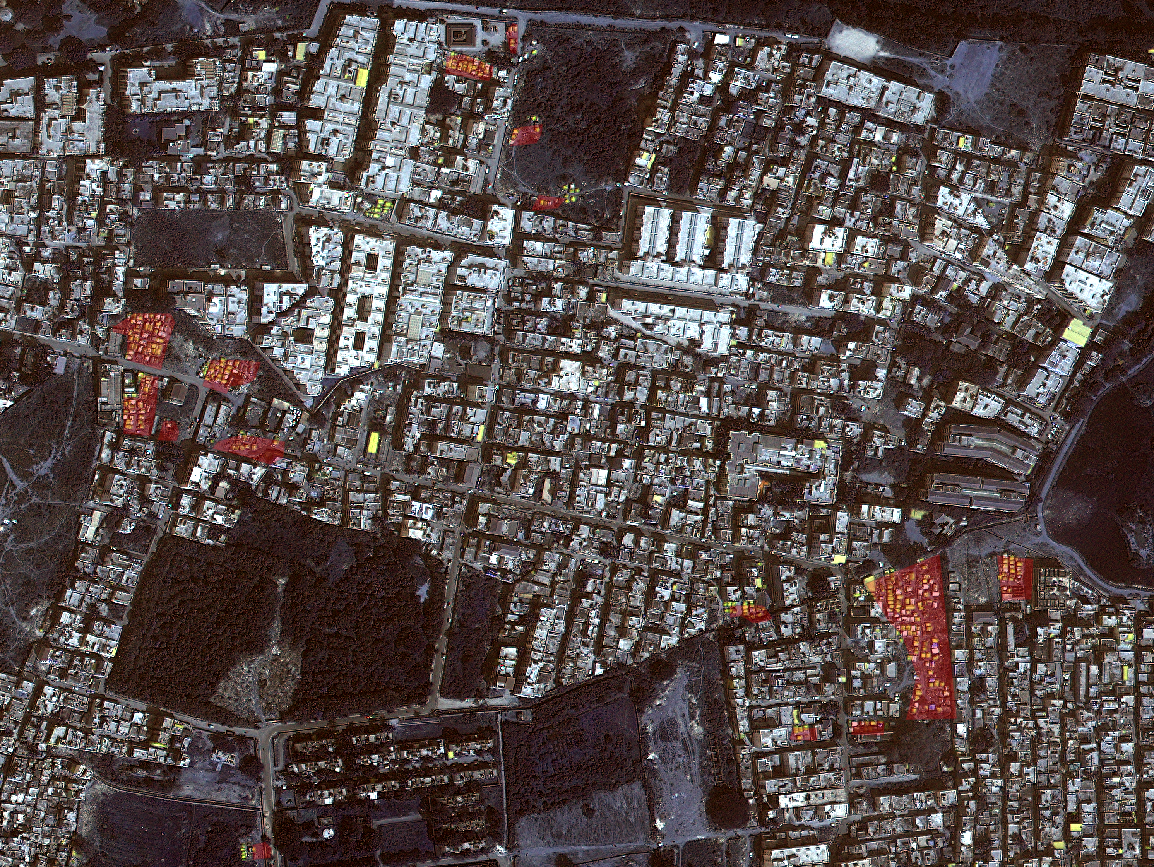
\includegraphics[width=\linewidth]{images/section_3}
%  \caption{Dense informal area in Bangalore, the red patches indicate informal
%  settlements}
%  \label{fig:section_3}
%\end{figure}

\begin{figure}
\centering
\begin{tabular}{cc}
  \subfloat[Section 1]{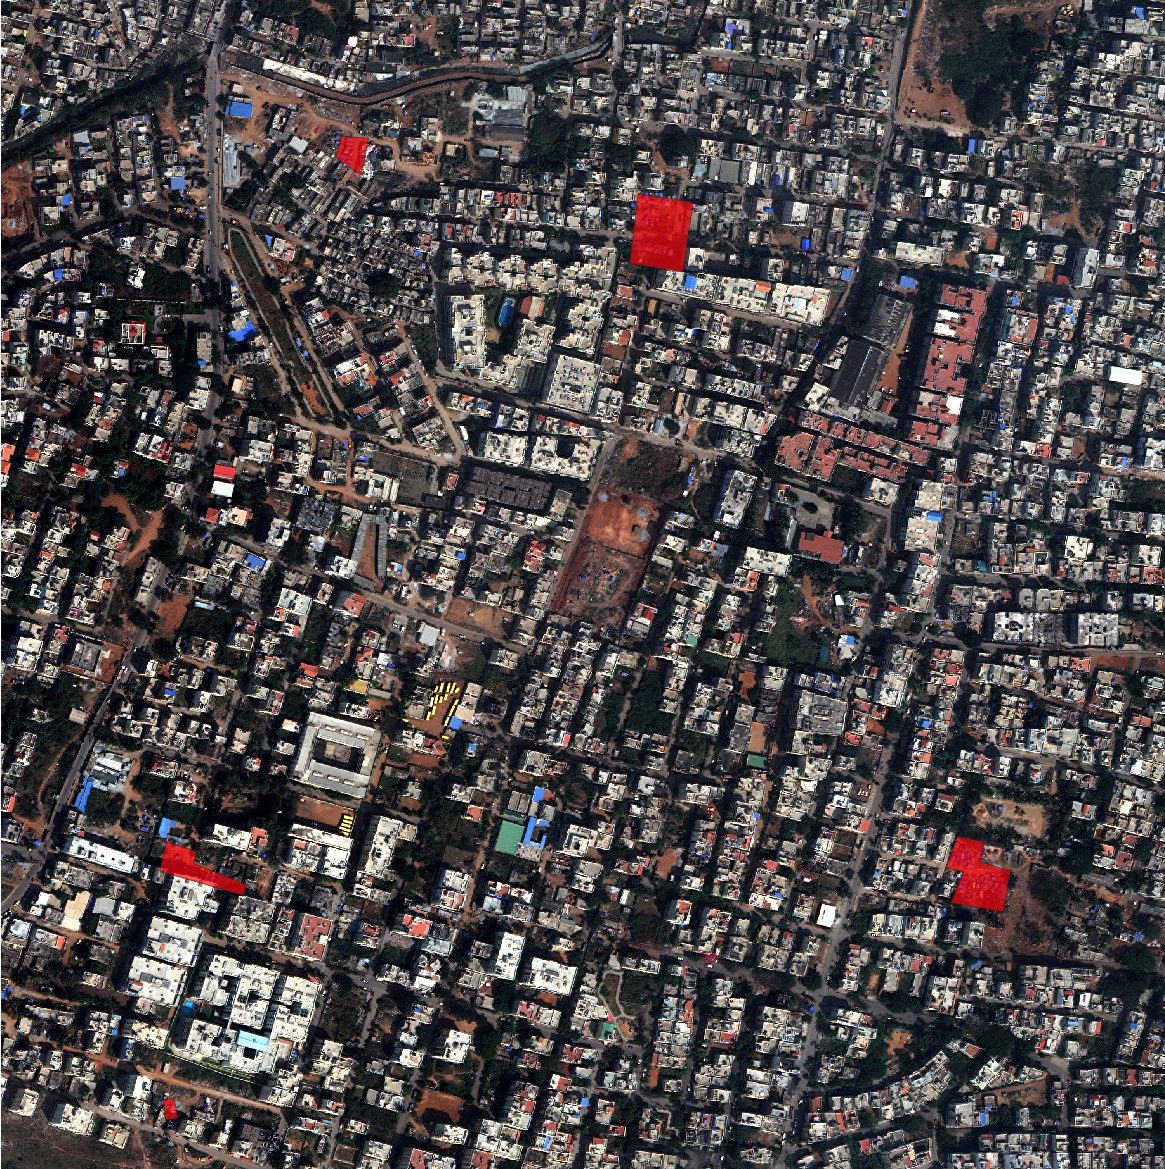
\includegraphics[width=6.2cm, height=5cm]{images/section_1_gt}}&
  \subfloat[Section 2]{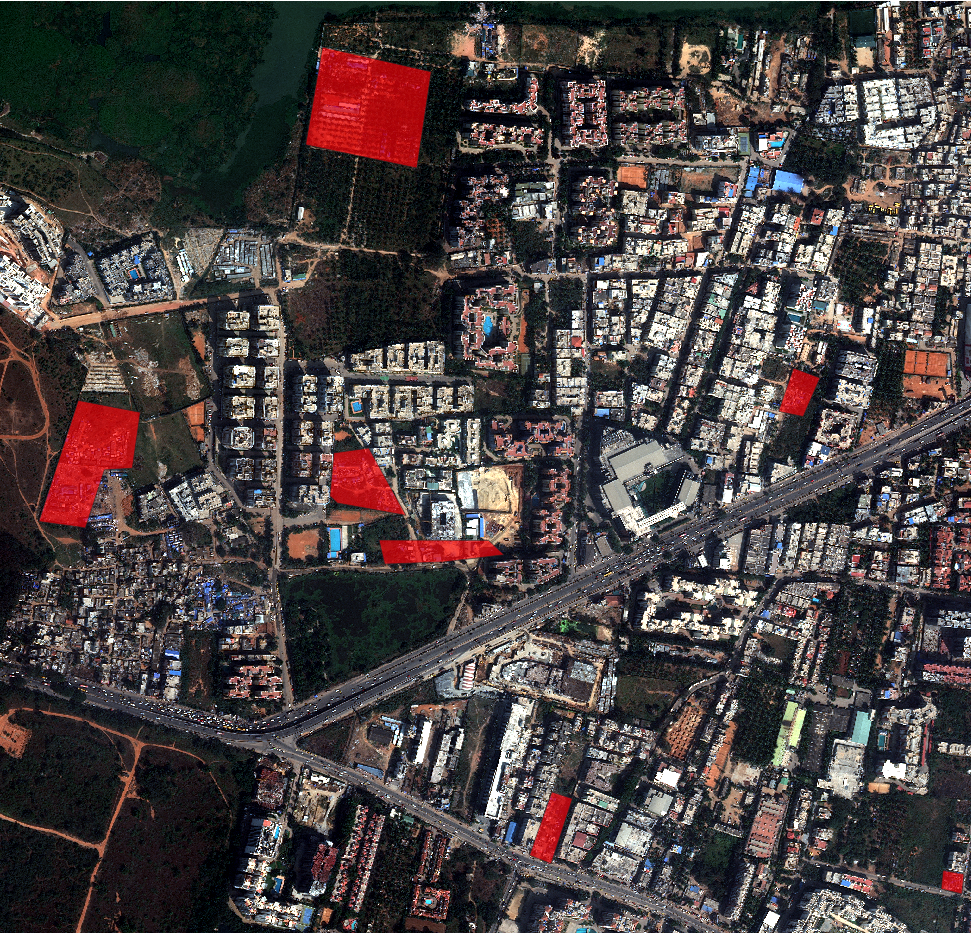
\includegraphics[width=6.2cm, height=5cm]{images/section_2_gt}}\\
  \subfloat[Section 3]{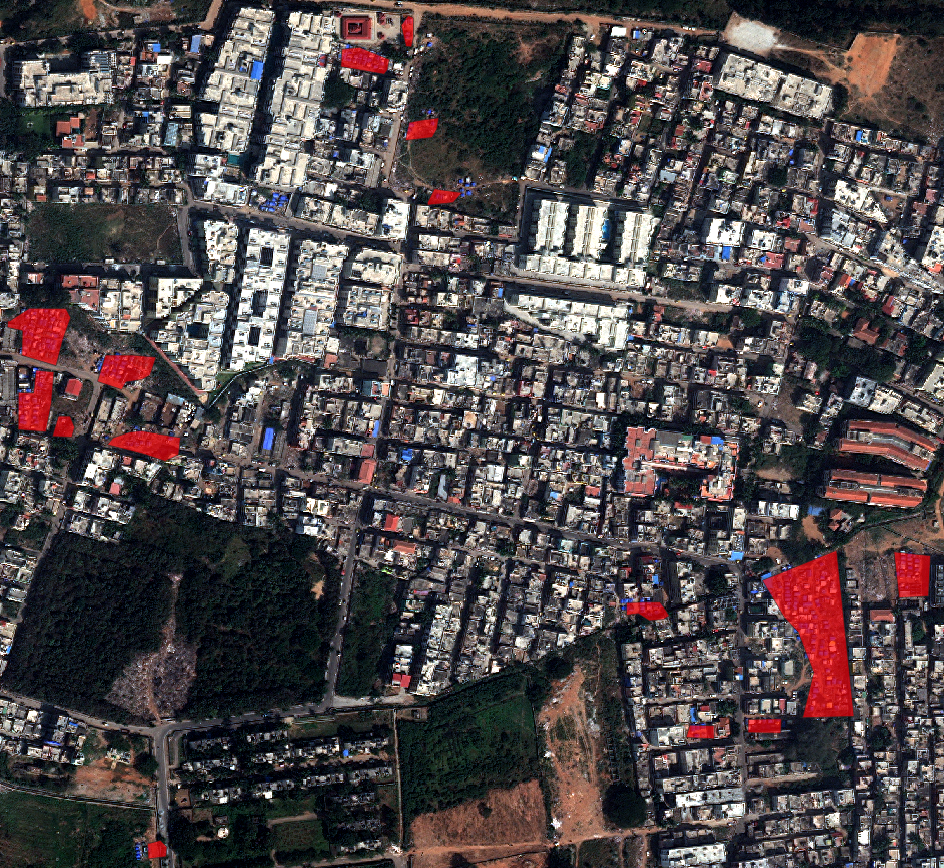
\includegraphics[width=6.2cm, height=5cm]{images/section_3_gt}}&
  \subfloat[Location of Sections]{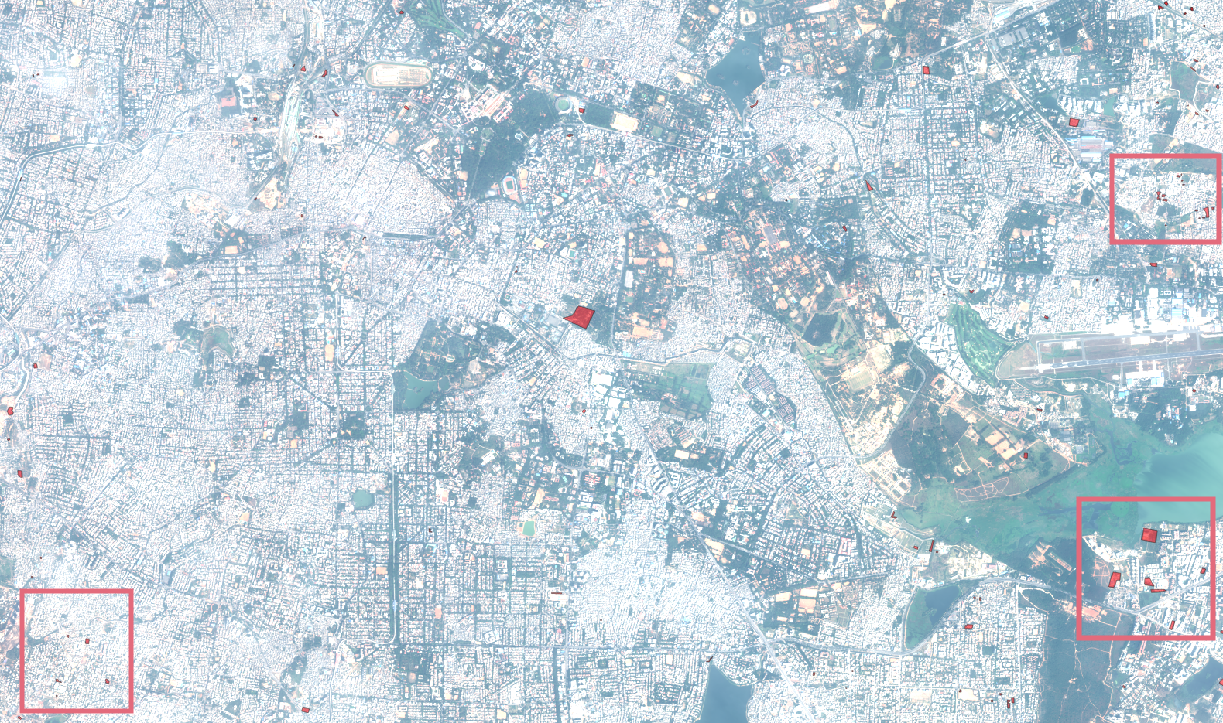
\includegraphics[width=6.2cm]{images/west-bangalore_sections}}
\end{tabular}
\caption{The images used for evaluation and classification}
\label{fig:sections}
\end{figure}



\section{Previous Work}

There have been multiple studies concerning the detection of informal
settlements using remote sensing in the last decade \cite{kuffer2016slums}.
Informal settlements in the proximity of cities have been studied throughout
the globe using remote sensing imagery, e.g. Colombo \cite{colombo},
Johannesburg \cite{williams2016automatic}, Accra \cite{accra}, Mumbai
\cite{mumbai}, and Hyderabad \cite{hyderabad}. There are numerous
characteristics that are suitable to differentiate between formal and informal
settlements. This could, for example,  be the number vegetation, the width of
the roads, the size and orientations of dwellings \cite{owen2013approach}.

In general, there is a shift towards the usage of objects for the
classification of geographical features. This is broadly known as Geographic
Object-based imaga analysis or GEOBIA \cite{hay2008geographic}.Due to the
increase in availability of remote sensing high resolution imagery, it became
feasible to distinguish individual objects on a large scale.  This allows for
the interpretation of geographical imagery with individual objects at its
basis.  As a result, the characterization of regions may be based on the type
of objects that inhabit it.  To illustrate, a study classified rooftop objects
from aerial imagery of an informal settlements in Johannesburg to gather
demographic information as an alternative to traditional ground based survey
\cite{williams2016automatic}.


Our study continues partly on the work performed by Graesser et al.  A study
from 2012 conducted by Graesser et al  investigated similar
problem, the characterization of formal and informal neighborhoods.  This study
uses a collection of different features to capture the difference in
characteristics between formal and informal neighborhoods in urban
environments. Our research will evaluate if the results obtained by Graesser et
al translates well to different cities with imagery from a different
satellite. Beyond the replication of previous research, the features used by
Graesser will be extended by an additional feature. This feature will be
compared to the existing features in various measures. The features combined
will be used by a set of different classification algorithms to both assess the
performance of the feature set as well as the evaluation of various
classification algorithms.


% difference everything not informal automatically fromal


\section{Conventional Feature Extraction Methods}
Studies often use a combination of features in the detection of informal settlements. Our research will use methods for feature extraction that performed well in previous research \cite{graesser2012image}. The methods we use are the Histogram of Oriented Gradients (HoG) and Line Support Region (LSR) features. Both HoG and LSR are already implemented in a Python library. This library, called spfeas, that is based on the research Graesser \textit{et al.} conducted on the classification of formal and informal neighborhoods \cite{graesser2012image}. Besides these two features we design a new method that measures the difference 
in prevalence and distribution of road intersections between formal and informal areas. This is based on the belief that there is a difference in this aspect between formal and informal areas.

\subsection{Terminology}
The paper of Graesser \textit{et al.} \cite{graesser2012image} uses blocks of pixels instead of each individual pixel when extracting features from images.  This is to ease the computational load because the extraction methods used are
computationally quite expensive, especially LSR. These blocks of pixels are of 20 by
20 pixels in the paper. The size of these pixel blocks is referred to as the \textit{block size}. In our research, the block size will differ from
this value to evaluate the affect to the performance of the features.
In addition to blocks, the paper also uses a set of different scales for the
calculation of features. A scale specifies the pixels around a block that
are used for the calculation of that block. This allows blocks to be
spatially connected to the surrounding areas, which can increase the
performance of features.

\subsection{Histogram of Oriented Gradients}
% designed for only settlement detection
% as supporting feature
% theory part
% however, Graesser does work for differentiating
% picture for explaination?


The Histogram of Oriented Gradients was originally used for the detection of
man-made structures in images. The features retrieved from the histogram were
able to differentiate between natural and man-made sections in an image. This
approach of man-made structure detection relies on the difference in the
distrubution of gradients in a particular region of the image. Because man-made
structures are often consists of straight lines and regular forms, this
contrasts the irregular forms that are naturally formed. This difference in
appearance translates to a difference in the distribution of gradients in
man-made structures and nature.

In satellite images, the difference of the Histogram of Oriented Gradients
between nature and human settlements is quite large. Eventhough HoG was
originallly used for differentiating between nature and man-made structures,
the paper of Graesser et al was able to succesfully to use HoG between formal
and informal neighborhoods. The paper uses the disparate spatial distribution of
buildings in formal and informal regions. The
placement of houses in formal regions are often placed in a regular pattern
with fixed orientations. Informal areas, in contrast, are usually constructed
without a design or regular pattern. This difference in regularity is
a characteristic that can be used for classification of formal or informal
settlements.

The order of regularity of an area can be captured using the number of
orientations in which buildings are constructed. Few distinct orientations suggest
a formal settlements while many orientations suggest informal. The orientations
of buildings are calculated using the gradients returned by the application of
a binary filter on the image. The gradients are quantized into a set of
orientations or bins. This results in a histogram commonly named the Histogram
of Oriented Gradients. High peaks in the HoG correspond to a multitude of
similar gradients, thus uniformity in the image. Since uniformity is linked
to formal settlements, high peaks in the histogram correlate with formal
settlements. The informal settlements, on the other hand, are characterized by
the absence of peaks in the HoG due to the multitude of different gradients
caused by the irregular placement of buildings.

Applied in practice, the paper from Graesser et al extracts five
characteristics from the HoG: two types of mean, variance, skew, and
kurtosis. These properties of the histogram are used as features to
describe the histogram and differentiate between formal and informal regions.
These 5 features will be calculated for every color band of the image,
resulting in a grand total of 15 features for the Histogram of Gradients.
According to the results presented in the paper, these 15 features alone could
result in an accuracy of 65 to 75 percent. It must be noted, however, that this feature was applied to specific regions where the visual difference between formal and informal was substantial, which is often not the case.

\subsection{Line Support Region Features}

The formality of regions can be for a part be determined by observing the
spatial distribution of neighborhoods. In the same manner as HoG characterized
areas by the orientation their buildings, neighborhoods, alternatively, can be
characterized by the size of their buildings. Informal settlements generally
lack the presence of large buildings in contrast with formal regions. The size
of constructions can be characterized using the Line Support Region (LSR)
features \cite{unsalan2004classifying}. Likewise to HoG, LSR utilizes gradients
calculated from remote sensing imagery. LSR uses the fact that straight lines
have uniform gradients. In practice, natural photographs hardly contain
perfectly straight lines, which results in similar but non uniform gradients of
lines. Therefore, LSR uses groups similar gradients to represent a line in
images to detect semi straight lines in images \cite{burns1986extracting}.

The LSR is implemented in spfeas in accordance to the paper of Graesser \textit{et al.} \cite{graesser2012image}. The paper uses three statistical features extracted
from the LSR, these are: line length entropy, mean, and entropy of line
contrasts. Together with three color bands, this brings the total to nine
features for a single scale. Using only LSR features and scales 50, 100, and 200, the paper achieved an accuracy of 60 to 75 percent.



\section{Method}


\subsection{Data}

The image data used are captured by the earth observation satellite WorldView3
owned by DigitalGlobe. The WorldView3 satellite produces multiple categories of
imagery with varying degrees of resolution. The panchromatic images have
a resolution of 0.31 meter in contrast to  the multiband images have
a significantly lower resolution of
1.24 meter. The project uses pansharpened images, which combines the high
resolution panchromatic- and the low resolution multiband images to create
high resolution RGB images.

The content of the images contain regions of Bangalore, which is the capital
city of the indian state of Karnataka, located in south central India. The
population of the city is over ten million and is recognized as a mega city.
Banglore is known to have problems concerning informal settlements. According
to a report from 2012, there are 862 reported slums in the city


\begin{figure*}
  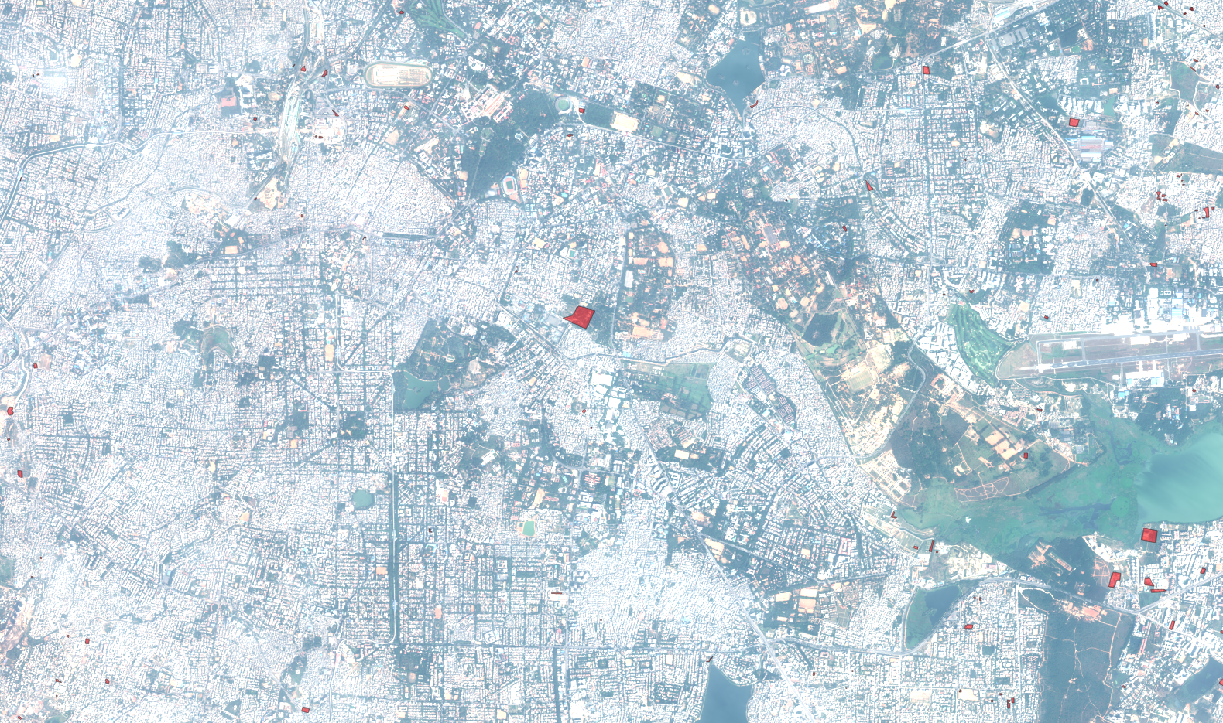
\includegraphics[width=\linewidth]{images/west-bangalore}
  \caption{A part of western Bangalore, the red patches indicate informal
  settlements}
  \label{fig:west-bangalore}
\end{figure*}

\subsection{Challenges}
The distinction between formal and informal regions is often quite challenging,
in part due to the vagueness of borders between the regions. The border between
formal and informal regions often resembles more of a spectrum than a clear cut line.
Besides border difficulties, some areas are not designated as informal, while
still posessing characteristics of an informal region. This results in
a dataset with noise and inconsistency.  All in all, the binary classification
of a region encounters difficulties when applied in practice. 


Another challenge encountered in this field is the scarcity of informal
settlements.  Eventhough Banglore  has an abundance of informal settlements,
the fast majority of land is identified as formal area's. Figure
\ref{fig:west-bangalore} shows a part of western Bangalore where it is clear
that informal settlements are sparce and distributed throughout the city. As
a result, the dataset of formal and informal regions becomes quite skewed.
Furthermore, because everything that is not informal is automatically
considered formal, the formal regions have a large amount of variance of visual
properties.  To illustrate: lakes, forrests, and fields fall in the same
catagory as formal residential and industrial areas while the visual
characteristics are significantly different. The diverse content of the formal
set of visual characteristics might hinder the effectiveness of differentiating
between formal and informal regions. 

To reduce the skewedness between informal and formal, only subsections of Figure \ref{fig:west-bangalore} are
used where the proportion formal to informal is less one-sided. An example of
such a region is Figure \ref{fig:section_3}. A smaller difference in formal
informal ratio allows for a better understanding of the effectiveness of
various features. The features are assesed using these area's 

\begin{figure}
\centering
  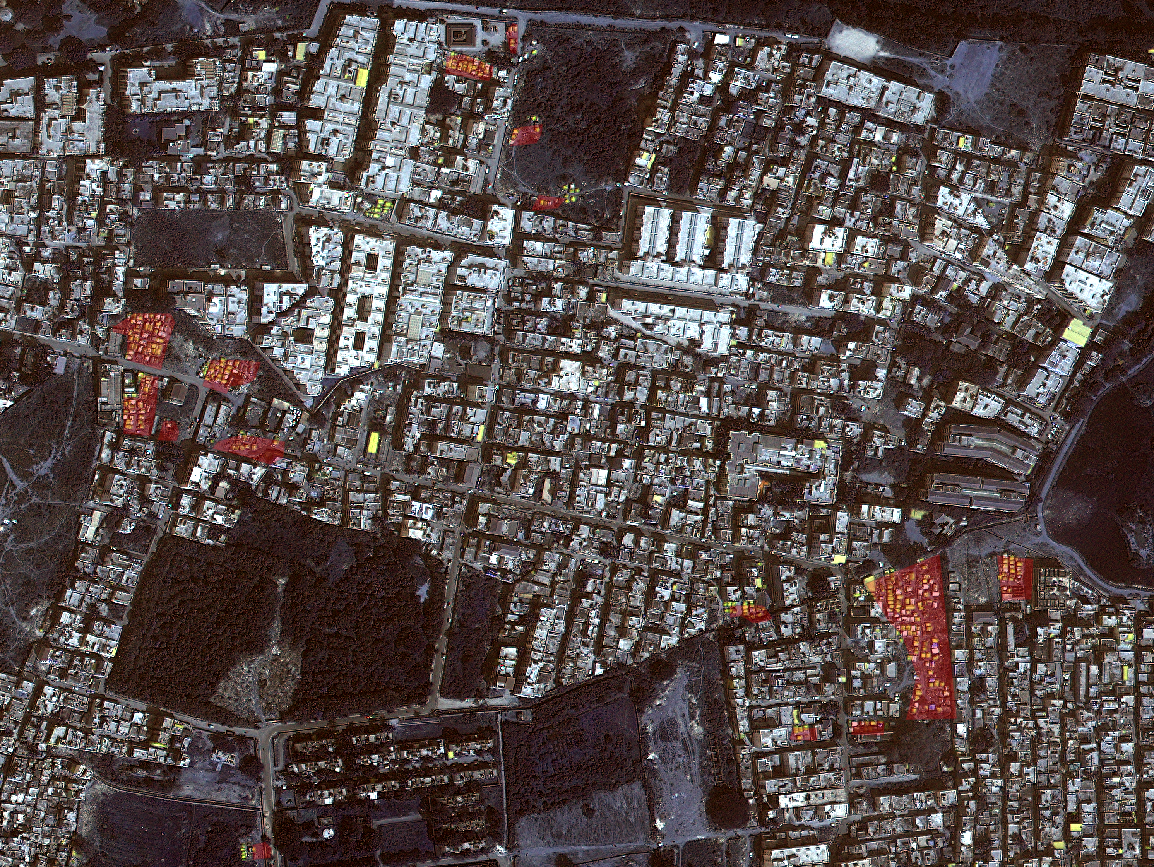
\includegraphics[width=\linewidth]{images/section_3}
  \caption{Dense informal area in Bangalore, the red patches indicate informal
  settlements}
  \label{fig:section_3}
\end{figure}

\subsection{Feature Evaluation}
An important part is the evaluation of the value of estimation that a certain
feature posesses. This allows to conclude if a certain feature is useful in the
discrimination between formal and informal. The use of a set of features allows
for a more solid estimation compared to a single feature by itself. 

The measure of predictive value of a feature is visualized using a boxplot and
the spatial distribution of values. A boxplot for a certain feature, consists
of two classes: the formal and informal class. To latter belong chunks of
pixels that are situated inside formal settlements. The former contains chuncks
that are not within informal regions. In the case that a feature is
distinctive, the distribution of the values in the two classes will be
different. The boxplot visualizes the difference in distribution well, showing
the usefulness of a feature.




\section{Feature Evaluation}

In order produce a functioning classifier, the predictive value of the features
must be evaluated. This assesses wether a certain feature is useful in the
discrimination between formal and informal. The evaluation requires the
knowledge of what parts in a satellite image are formal and informal to create
a distinction between the two classes. This knowledge is represented in
a ground truth, this is a mask covering the satellite image indicating the
informal regions.

The mask is used to divide each block of pixels into the two classes, formal
and informal. Each block has a vector of values, also called features,
characterizing that particular block. Because the blocks are grouped together,
the features associated with the same class are grouped together as well. This
allows for the analysis of the distribution of the features in both classes. If
the distribution of a certain feature varies quite distinctly between the two
classes, this indicates as a suitable candidate for classification of informal
regions.

The groundtruth mask is constructed using a vector file containing the
boundaries of informal areas. The boundary file is rasterized and applied on
top of the satellite image, creating a mask of the informal settlements.
Because classification and feature calculation is performed on blocks instead
of pixels, the pixel based mask transformed into a block based mask. In this
mask, every pixel represents a block where the zero represents formal and one
represents informal. This effectively creates a ground truth.  

The predictive value of a feature can be visualized using a boxplot of the two
classes. When a feature is distinctive on its own, the distribution of the
values in the two classes will be different. The data used for the evaluation
comes from three small sections of the image. As priorly mentioned, this
creates a more even division of classes which should provide a more accurate
evaluation of the selected feature.

The features will be calculated for every image at different block sizes and
scales. Because block size and scale impact the predictiveness of a feature,
various combinations are used to discover the most favorable combination.

% TODO: insert concatenated image of the three sections

%Eventhough there might not be
%a significant difference between two distribution, by using multiple features
%in combination, the grand total might more distinctive that the sum of its
%parts. 

\subsection{Histogram of Oriented Gradients}

In the analysis of the historgram used block sizes of 20, 40, and 60 combined
with scales of 50, 100, 150, and 200. These combinations should capture the
difference that either an increase of block size or scale causes to the
predictiveness of a feature. For visualization purposes, only a single feature
of the 15 features of HoG of a single section is displayed here. This feature
is the most distinct between formal and informal. The other two sections are
comparable to the section used here. Moreover, not all combinations of the
block sizes and scales are presented here, only a few examples which illustrate
the distinctiveness of the features of the Histogram of Oriented Gradients.

\begin{figure}
\begin{tabular}{cc}
  \subfloat{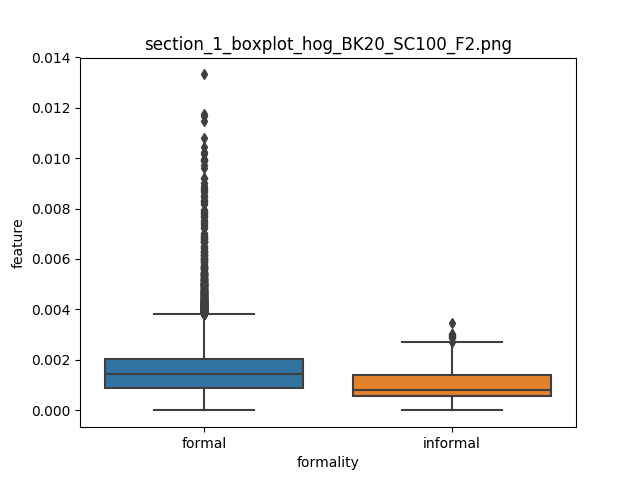
\includegraphics[width=4cm]{images/HoG/inc_bk/section_1_boxplot_hog_BK20_SC100_F2}}&
  \subfloat{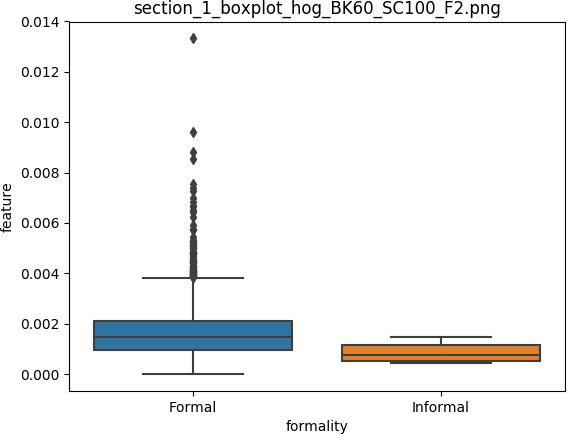
\includegraphics[width=4cm]{images/HoG/inc_bk/section_1_boxplot_hog_BK60_SC100_F2}}\\ 
  \subfloat{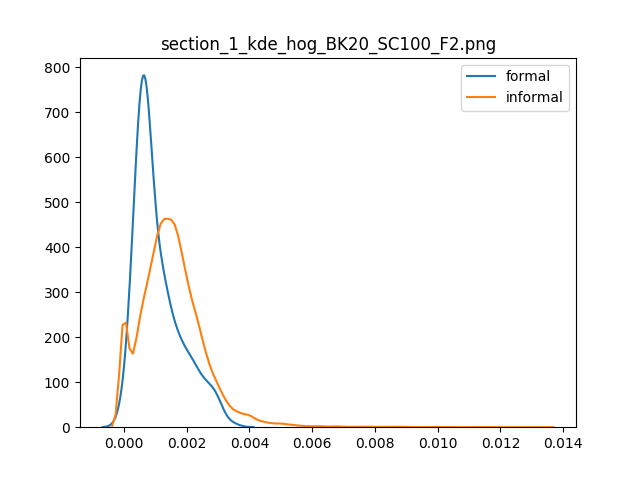
\includegraphics[width=4cm]{images/HoG/inc_bk/section_1_kde_hog_BK20_SC100_F2}}&
  \subfloat{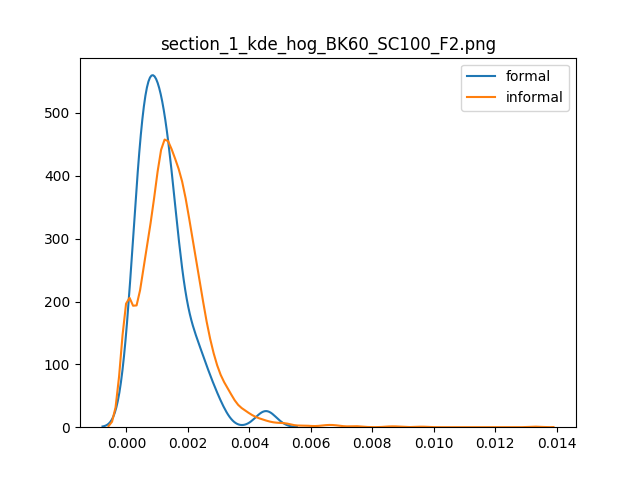
\includegraphics[width=4cm]{images/HoG/inc_bk/section_1_kde_hog_BK60_SC100_F2}}
\end{tabular}
\caption{The effect of increased block size on a HoG feature. From left to
right: a block size of 20 and 60 respectively.}
\label{hog_inc_bk}
\end{figure}

Figure \ref{hog_inc_bk} shows the effect that an increased block size has on
the distribution of values in both classes. This example uses a constant scale
of 100 pixels and a variable block size of 20 and 60 pixels. The experiment
with a block size of 40 is performed as well, but is ommited from the figure to
keep the results brief. A more comprehensive visualization of the evaluation
can be found in the appendix. It seems that the block size, in this case, does
not influence the both distrutions significantly. As a result an increase in
the size of a block will have little influence on the predictive value of the
HoG.

\begin{figure}
\begin{tabular}{cc}
  \subfloat{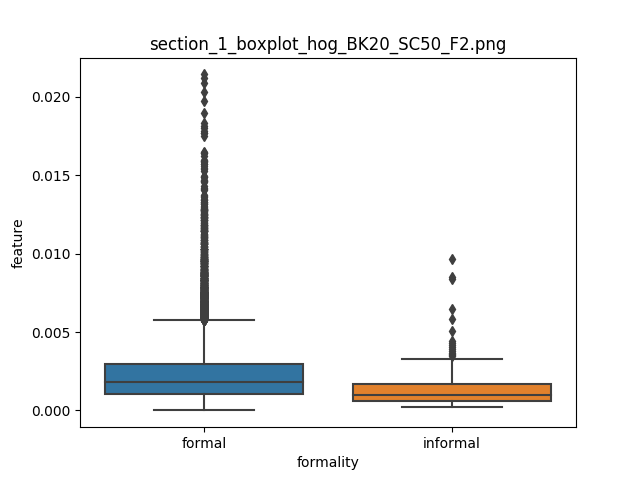
\includegraphics[width=4cm]{images/HoG/inc_sc/section_1_boxplot_hog_BK20_SC50_F2}}&
  \subfloat{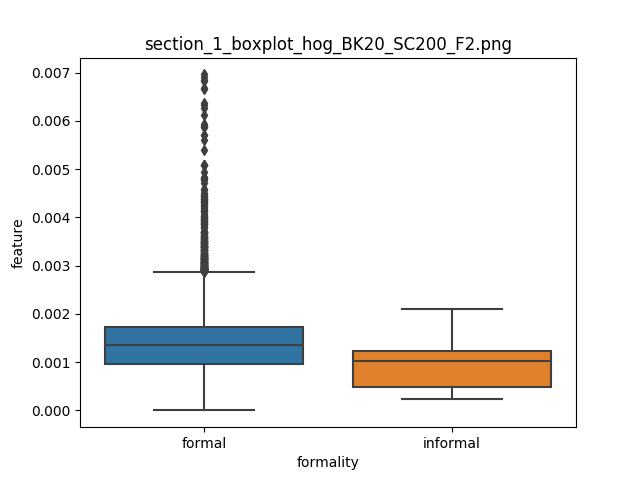
\includegraphics[width=4cm]{images/HoG/inc_sc/section_1_boxplot_hog_BK20_SC200_F2}}\\
  \subfloat{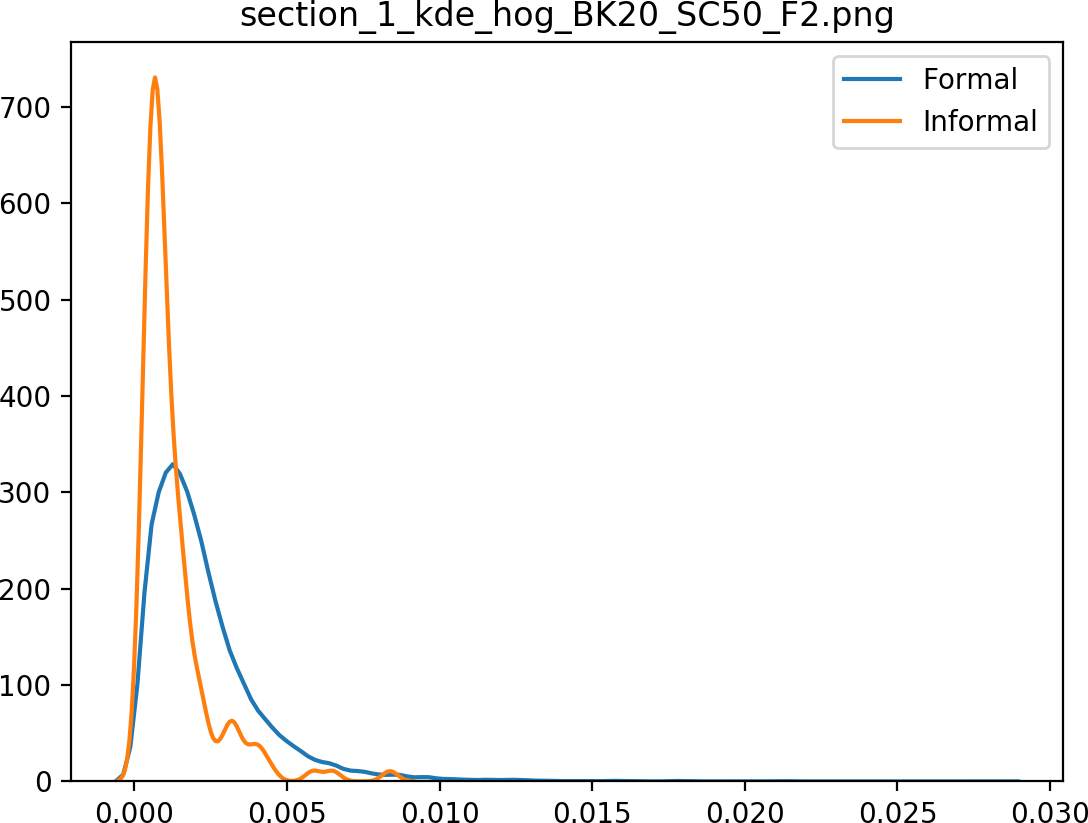
\includegraphics[width=4cm]{images/HoG/inc_sc/section_1_kde_hog_BK20_SC50_F2}}&
  \subfloat{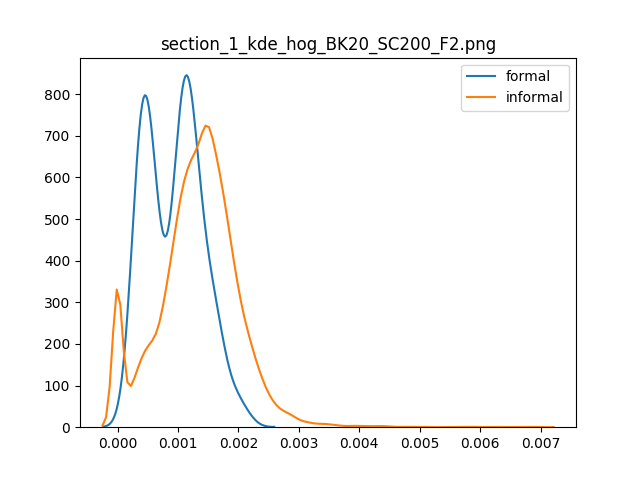
\includegraphics[width=4cm]{images/HoG/inc_sc/section_1_kde_hog_BK20_SC200_F2}}\\
\end{tabular}
\caption{The effect of increased scale on a HoG feature. From left to
right: a scale of 50 and 200 respectively}
\label{hog_inc_sc}
\end{figure}

Figure \ref{hog_inc_sc} illustrates the effect of increased scale on a constant
block size. It seems to indicate that an increased scale leads to an increased
separatation of the two distribution, thus increasing the predictiveness of the
feature.

\subsection{Line Support Region}

Similar to the analysis of the Histogram of Oriented Gradients, the analysis of
Line Support Region uses a combination of different block sizes and scales.
Unlike HoG, however, the scale 200 is not included due to the high
computational cost. 


% feature evaluation
%
% classification methods
%
% classification results (using the features)
%
% discussion: - features
%             - classification algo's
%             - other


\clearpage

\printbibliography

\end{document}

Gradient-Magnitude-Based Support Regions in Structural Land Use Classification
